\section{Chapter 8: Visual Objects and Data Objects}
\graphicspath{ {pngs/ch8/} }

\secttoc

This chapter is far from the concepts of extraction of information from the
retina. Once an object is recognized from the set of features, the rest of the
brain's systems can process it: visual feedback loops, language, action.
Little or no irrelevant information is processed, therein lies the power of
human visual thinking.

\begin{mdframed}\begin{multicols}{2}
\subsection{Image-Based Object Recognition}
\begin{compactdesc}
    \item[Image-based object recognition] recognition, not recall. We can
        rather reliably detect objects we have seen before.
    \item[RSVP] rapid serial visual presentation -- pictures shown at 10 per
        second, people know if a certain object is present
    \item[3D objects] generally recognized according to same view they were
        introduced.
    \item[Priming] even a fleeting meaningless encounter with a visual
        similar can prepare you to recognize the object again.
    \item[Searching an Image Database] RSVP could help. Video sped up 64x
        seems optimal.
    \item[Life Logging] recording one's life on video is not the same as
        remembering: it would take much time to recall the details of a truly
        forgotten event. Can support memory to some extent.
\end{compactdesc}
\end{multicols}\end{mdframed}

\begin{mdframed}\begin{multicols}{2}
\subsection{Structure-Based Object Recognition}

    \begin{figure}[H]
        \centering
        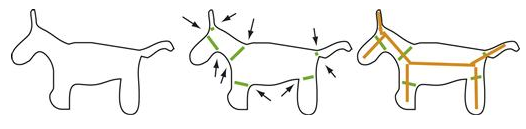
\includegraphics[width=0.4\textwidth]{contours_donkey.png}
        \caption{Concave sections define a structural skeleton.}
    \end{figure}
\begin{compactdesc}
    \item[Structure-Based Object Recognition] visually distinct 3D views can
        be recognized as the same object.
    \item[Geon theory] a hierarchical set of processes: edges,
        axes/blobs/vertices, finally 3D primitives cones/cylinders/boxes (Geons)
        are recognized
    \item[Geon] 3D primitive: cone, cylinder, box, sphere
    \item[Silhouettes] at some level, these excite the same neurons an actual
        3D object does. Canonical views recognized easily. Theory:
        2D contours segment image into component solids. Simplified line
        drawings easier to see than photographs.

\end{compactdesc}

    \begin{figure}[H]
        \centering
        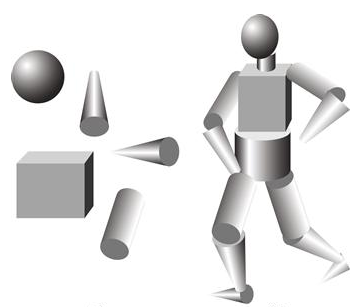
\includegraphics[width=0.6\linewidth]{geons.png}
        \caption{Geons}
    \end{figure}
\end{multicols}\end{mdframed}





\begin{mdframed}\begin{multicols}{2}
\subsection{Object-Based Diagram}
\begin{figure}[H]\centering
    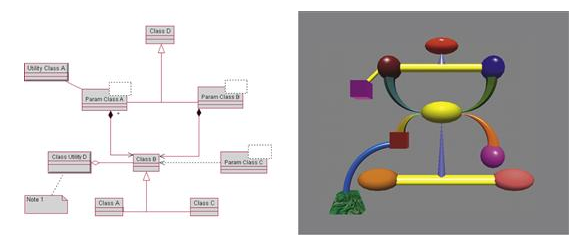
\includegraphics[width=0.4\textwidth]{uml_old_vs_geons.png}
    \caption{Standard UML diagram on the left vs. a geon diagram representing
    the same relationships.}
\end{figure}

\begin{compactdesc}
    \item[Object Display] many variables represented as a ``single contoured
        object.'' Most effective when graphical representations have a natural
        or metaphorical meaning.
    \item[Disadvantage] lack generality, object must have meaningful mapping to
        data.
    \item[Geon diagram] geons make good elements: color/texture can be
        attributes.
    \item[Faces] universally recognized; cannot be generalized to any data or
        any variable ranges due to emergent expressions generated by some
        arbitrary points of data. Chernoff faces not in general use.
\end{compactdesc}

\begin{figure}[H]\centering
    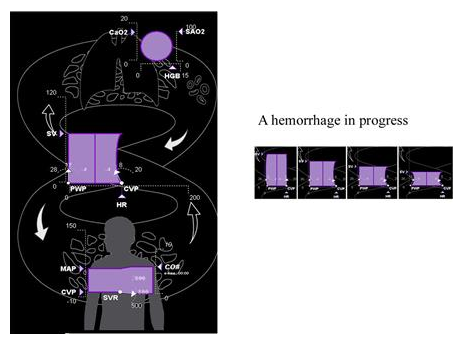
\includegraphics[width=\linewidth]{object_based_anesthesiologist.png}
    \caption{Object-based diagram. Height is volume per heart beat, width is bpm,
    curving of left- and right-hand sides indicates pressure on left and
    right sides of heart. Errors reduced by 66\%.}
\end{figure}
\end{multicols}\end{mdframed}

%\begin{figure}[H]\centering
%    \includegraphics[width=0.4\textwidth]{.png}
%    \caption{.}
%\end{figure}
%\begin{figure}[H]\centering
%    \includegraphics[width=0.4\textwidth]{.png}
%    \caption{.}
%\end{figure}




\begin{mdframed}\begin{multicols}{2}
\subsection{Coding Words, Images}
\begin{compactdesc}
    \item[Logogens] mental representation of language
    \item[Imagens] mental rep. of visual information
    \item[Dual coding theory] imagens are separate from logogens
    \item[Mental image] Imagining and changing the position and size of
        mental images activates similar neurons.
        Visual object processing and recognition are part of
        the same process.
\end{compactdesc}


\subsection{Labels, Concepts}
\begin{compactdesc}
\item[High-level object concepts] set of objects labeled with uses, relations,
    properties. Takes time to develop this network.
\item[Object categorization] see spoon: verbal label activated. Object file:
    links object and its many attributes
\item[Canonical views] not all views are equally easy to recognize
\item[Categorical object] not all categories can be represented by a simple
    icon
    \midrule
\item[Concept maps] nodes are concepts, links are relationships. It is
    important for students to integrate new knowledge into this network.
    Can be helpful in communication visualizations.
\end{compactdesc}
\end{multicols}\end{mdframed}


\begin{mdframed}\begin{multicols}{2}
\subsection{Icons, Words, Symbols}
\begin{compactdesc}
\item[Symbols] can be icons, words or abstract objects.
\item[Pictorial icons] best for pedagogy.
\item[Word or abstract] symbols: choose based on cognitive efficiency.
\item[Static links] integrating text into a static diagram? Consider Gestalt
    principles.
\end{compactdesc}

\subsection{Scenes and Scene Gist}
\begin{compactdesc}
    \item[Rapid categorization] occurs with scenes, not just objects.
        Within 100ms, you know if its a beach, street, interior\dots
    \item[Scene gist] important because what we see depends on context
    \item[Priming] positive: improved categorization, negative: alternative
        interpretations weakened
    \item[Trace theory] when activity is completed, corresponding neural
        pathways become strengthened. Faster at automatic classification; less
        interpretation.
\end{compactdesc}

\begin{figure}[H]\centering
    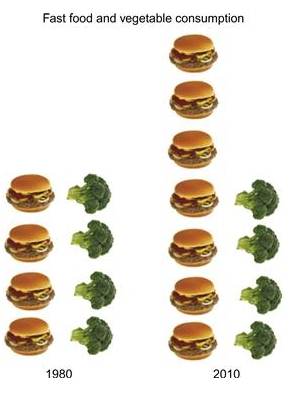
\includegraphics[width=0.35\linewidth]{pictorial.png}
    \caption{Example visualization using pictorial icons.}
\end{figure}

\begin{figure}[H]\centering
    
\includegraphics[width=0.5\linewidth]{similar_pairs.png}
    \caption{Pairs of similar objects with different uses.}
\end{figure}

\end{multicols}\end{mdframed}





